We evaluated Bounded Approximate SDP on the didactic domains:

\MarsRoverUni:
A unidimensional domain, where the position of the rover is a single continuous variable ($x$) and the goal of the rover is to take pictures at specific points. There is only one action $ move(a_x)$ with $a_x$ unbounded.
Description of the problem for instance rover1d2, there are two pictures points and taking pictures is recorded in two boolean variables ($tp_1$ and $tp_2$).
{\footnotesize
\begin{align*}
tp_1' &= 
(x>40) \wedge (x<60) &: 1\\
else &: 0\\
tp2' &= 
(x<-40) \wedge (x>-60) &: 1\\
else &: 0\\
x' &= x +a_x\\
R & = \begin{cases} \\
(tp1') \wedge (\neg tp1) \wedge (x > 50) &: 40 - 0.2*(x -50)\\
(tp1') \wedge (\neg tp1) \wedge (x < 50) &: 40 - 0.2*(50-x)\\
(tp1') \wedge ( tp1) &:  0.0\\
else & -2\\
\end{cases} &
\end{align*}}

\begin{figure}[h!t]
\center
\fbox{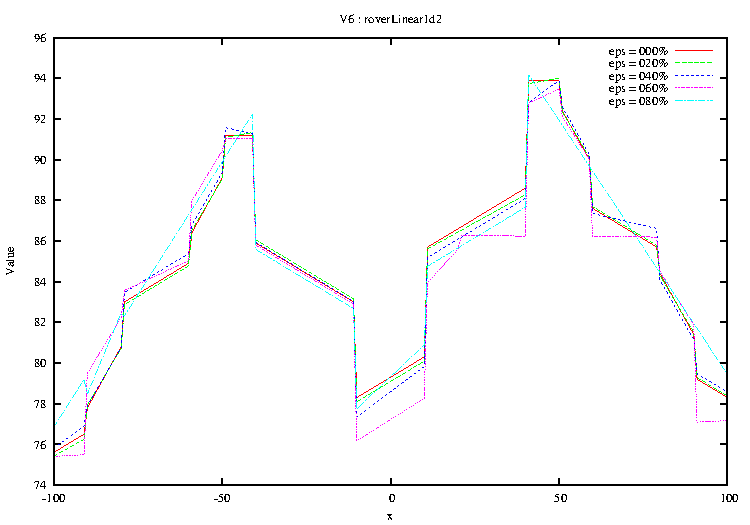
\includegraphics[scale=0.4]{Figures/rover1D/rover1d2V6.pdf} }
\caption{Value Function at Iteration 6 for rover1d2.}
\label{steplin} 
\end{figure}



\MarsRoverBi: In this version of \MarsRover there are no picture points as goals but the rover is expected to follow a path. In this the position is represented by a pair or continuous variables $(x,y)$. There is only one action, $move(a_x,a_y)$, where $|a_x|$ <10 and $|a_x|$ <10. The increasing value of $x$ and keeping $y$ close to zero is reward 

{\footnotesize
\begin{align*}
x' &= x +a_x\\
y' &= y +a_y\\
R & = \begin{cases}
(x > y +25) \wedge (x > - y  +25) \wedge (y >0) &: -10 + x -y\\
(x > y +25) \wedge (x > - y  +25) \wedge (y <0) &: -10 + x +y\\
else & -1\\
\end{cases}
\end{align*}}

\begin{figure}[tbp!]
\centering
\subfigure[Value at $6^{th}$ iteration for exact SDP.] {
	 \fbox{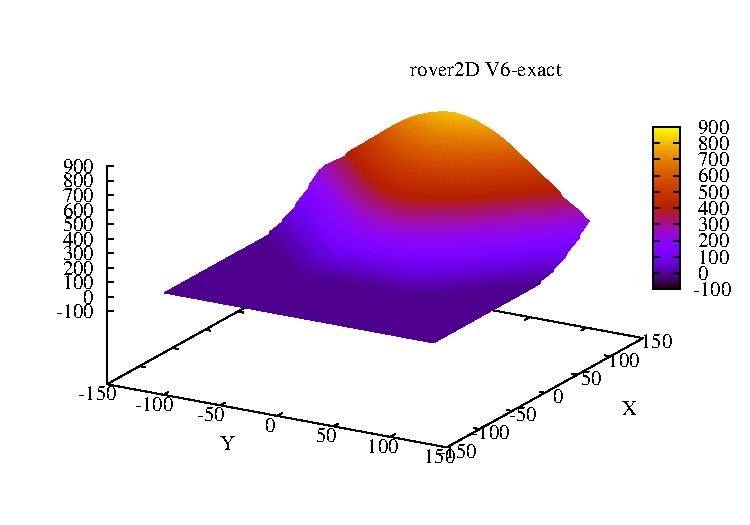
\includegraphics[width=0.22\textwidth, height=0.15\textwidth]{Figures/rover2D/rover2dV6-0.pdf}}
	 \fbox{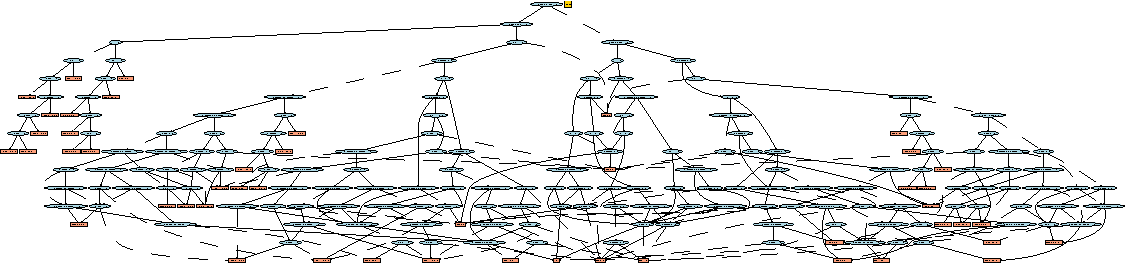
\includegraphics[width=0.22\textwidth, height=0.15\textwidth]{Figures/rover2D/rover2dV6-0xadd.pdf}}
	 \label{V6-0xadd}
}
\subfigure[Value at $6^{th}$ iteration for $5\%$ approximate SDP.] {
	 \fbox{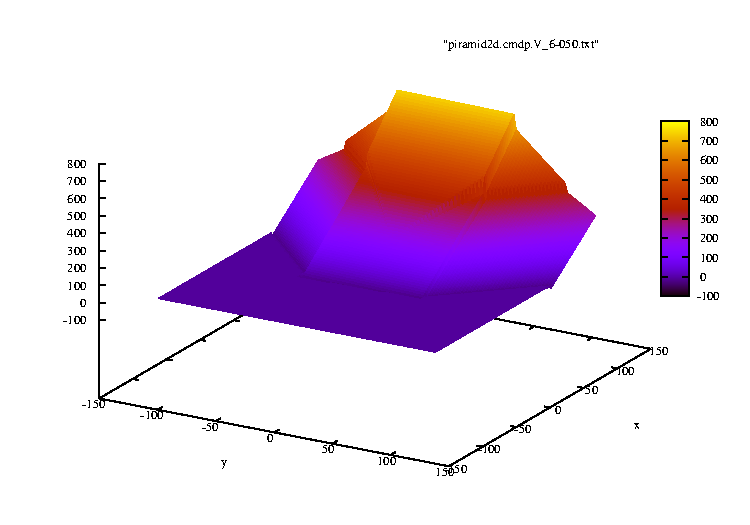
\includegraphics[width=0.22\textwidth, height=0.15\textwidth]{Figures/rover2D/rover2dV6-5.pdf}}
	 \fbox{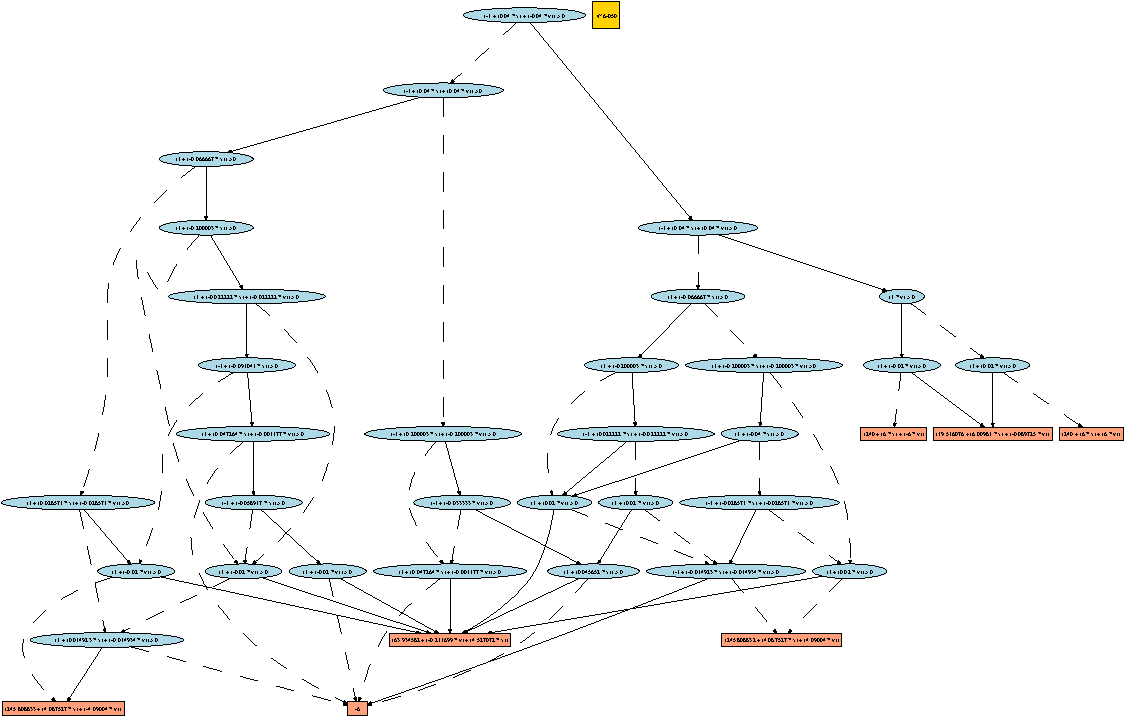
\includegraphics[width=0.22\textwidth, height=0.15\textwidth]{Figures/rover2D/rover2dV6-5xadd.pdf}}
	 \label{V6-5xadd}
}
\caption {\footnotesize
	Value function at iteration 6 for the \MarsRoverBi domain;
	{\it (top)} Exact value function; 	{\it (bottom)} Approximate value function with error bounded 5\% per iteration;
	{\it (right)} 3D Plots; {\it (left) XADD Diagrams}.
}
\label{fig:Mars2DV6}
\vspace{-5mm}
\end{figure}

\Invent:
A multidimensional continuous, in $n$-$\Invent$, there are $n$ continuous resources that can be bought and sold. There is a action $order$-$i$ for each resource, $ 1 \leq i \leq n$. The maximum amount of  each resource that is sold on one iteration depends on a stochastic demand variable $d$. 

{\footnotesize
\begin{align*}
action &  order-i:\\
d' &= 0.6\\
x_i' & = \begin{cases} 
(d') \wedge (x_i > 150) &: x_i + 200 - 150\\
(d') \wedge (x_i < 150) &:  200\\
(\neg d') \wedge (x_i > 50) &: x_i + 200 - 50\\
(\neg d') \wedge (x_i < 50) &:  200\\
\end{cases} \\
x_j' & = \begin{cases} 
(d') \wedge (x_j > 150) &: x_j - 150\\
(d') \wedge (x_j < 150) &:  0\\
(\neg d') \wedge (x_j > 50) &: x_j - 50\\
(\neg d') \wedge (x_j < 50) &:  0\\
\end{cases} \\
R & = \begin{cases} \\
(d') &: \sum_{k} {x_k' - x_k}\\
(tp1') \wedge (\neg tp1) \wedge (x < 50) &: 40 - 0.2*(50-x)\\
(tp1') \wedge ( tp1) &:  1.1\\
else & -2\\
\end{cases} 
\end{align*} }


\begin{figure*}[tbp!]
\centering
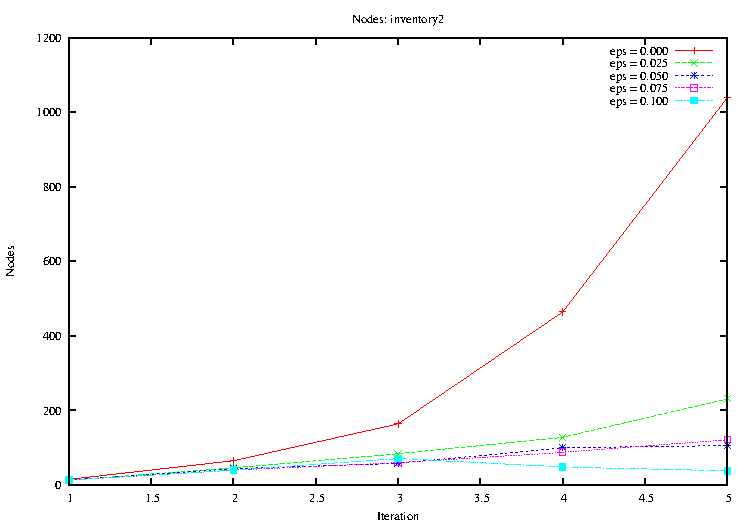
\includegraphics[width=0.30\textwidth]{Figures/inventory/invent2Nodes.pdf}
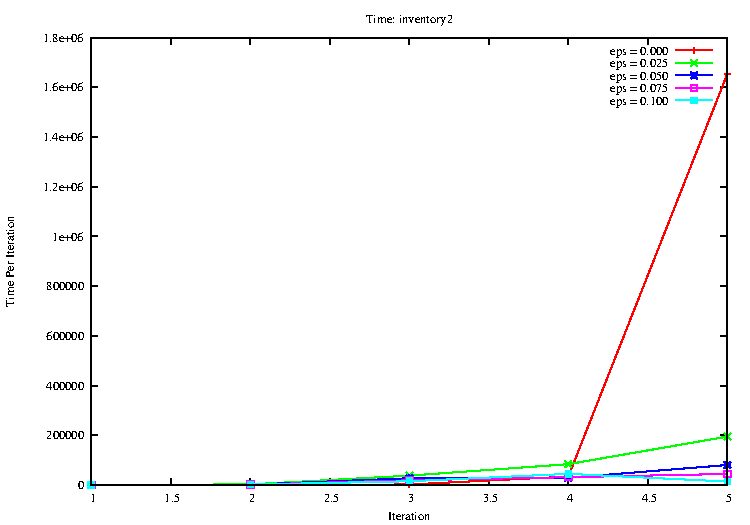
\includegraphics[width=0.30\textwidth]{Figures/inventory/invent2Time.pdf}
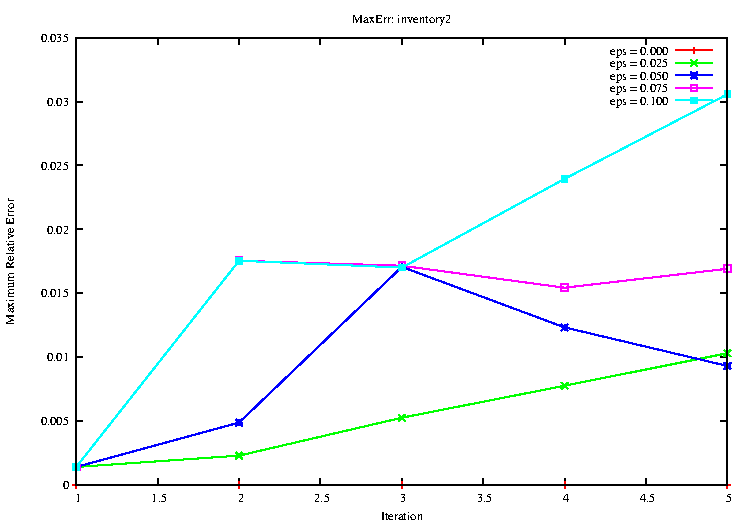
\includegraphics[width=0.30\textwidth]{Figures/inventory/invent2MaxErr.pdf}
\vspace{-2mm}
\caption{\footnotesize
{\it (left)}  $V^4(x,y,l=false)$\textsc{UAV Navigation} problem;
{\it (middle)} $V^7(l_1,d_1=false,d_2=false,d_3=false)$ \textsc{Reservoir Control} problem;
{\it (right)} $V^4(k,v,z=true,g=false)$ \textsc{Space Telescope Control} problem.
}
\label{fig:Value}
\vspace{-5mm}
\end{figure*}


